\section{认识时间序列}

\begin{definition}[时间序列]
    时间序列中的每个特殊点都与先前的数据点相关。
\end{definition}

人们通常使用一些简单的预测法：

\subsection{朴素预测法}

\begin{theorem}
    朴素预测法是时间序列预测中最简单的一种方法，它假设未来的值等于最近一个观测值。
    \begin{equation}
        \hat{y}_{t+1} = y_t
    \end{equation}
    其中，$\hat{y}_{t+1}$ 是对下一个时间点的预测值，$y_t$ 是当前时间点的实际观测值。
\end{theorem}

\subsection{简单平均值法}

\begin{theorem}[简单平均值法]
    简单平均值法是通过计算历史数据的平均值来预测未来的值。
    \begin{equation}
        \hat{y}_{t+1} = \frac{1}{n} \sum_{i=1}^{n} y_i
    \end{equation}
    其中，$n$ 是历史数据点的数量，$y_i$ 是第 $i$ 个观测值。
\end{theorem}

\begin{tips}
    它将下一个值视为先前所有值的平均数，但是这个方法的值可能并不都有用。

    因为可能你要预测今天的温度，只需要考虑七天内的温度即可，而不是一个月内的温度。
\end{tips}

\subsection{移动平均法}

为了解决上面这个方案的不足，移动平均法就诞生了。

\begin{theorem}[移动平均法]
    移动平均法是通过计算最近 $n$ 个观测值的平均值来预测未来的值。
    \begin{equation}
        \hat{y}_{t+1} = \frac{1}{n} \sum_{i=0}^{n-1} y_{t-i}
    \end{equation}
    其中，$y_{t-i}$ 是当前时间点 $t$ 向前推 $i$ 个时间点的观测值。
\end{theorem}

\subsection{加权移动平均法}

\begin{theorem}[加权移动平均法]
    加权移动平均法是对最近 $n$ 个观测值赋予不同的权重来预测未来的值。
    \begin{equation}
        \hat{y}_{t+1} = \sum_{i=0}^{n-1} w_i y_{t-i}
    \end{equation}
    其中，$w_i$ 是第 $i$ 个观测值的权重，满足 $\sum_{i=0}^{n-1} w_i = 1$。
\end{theorem}

\subsection{简单指数平滑法}

\begin{theorem}[简单指数平滑法]
    更大的权重被分配给更近期的观测结果，遥远的过去的观测值被赋予更小的权重。
\end{theorem}

\subsection{霍尔特线性趋势模型}

\begin{theorem}[霍尔特线性趋势模型]
    这个方法考虑了数据集的趋势。例如是递增或递减的，这个方法的预测函数是值和趋势的函数。
\end{theorem}

\subsection{霍尔特-温特斯（Holt Winters）方法}

\begin{theorem}
    该算法考虑了数据的趋势和季节性变化，例如酒店在周末订单数量更多，在工作日就会很低。
\end{theorem}

\section{ARIMA 模型}

\begin{figure} [H]
    \centering
    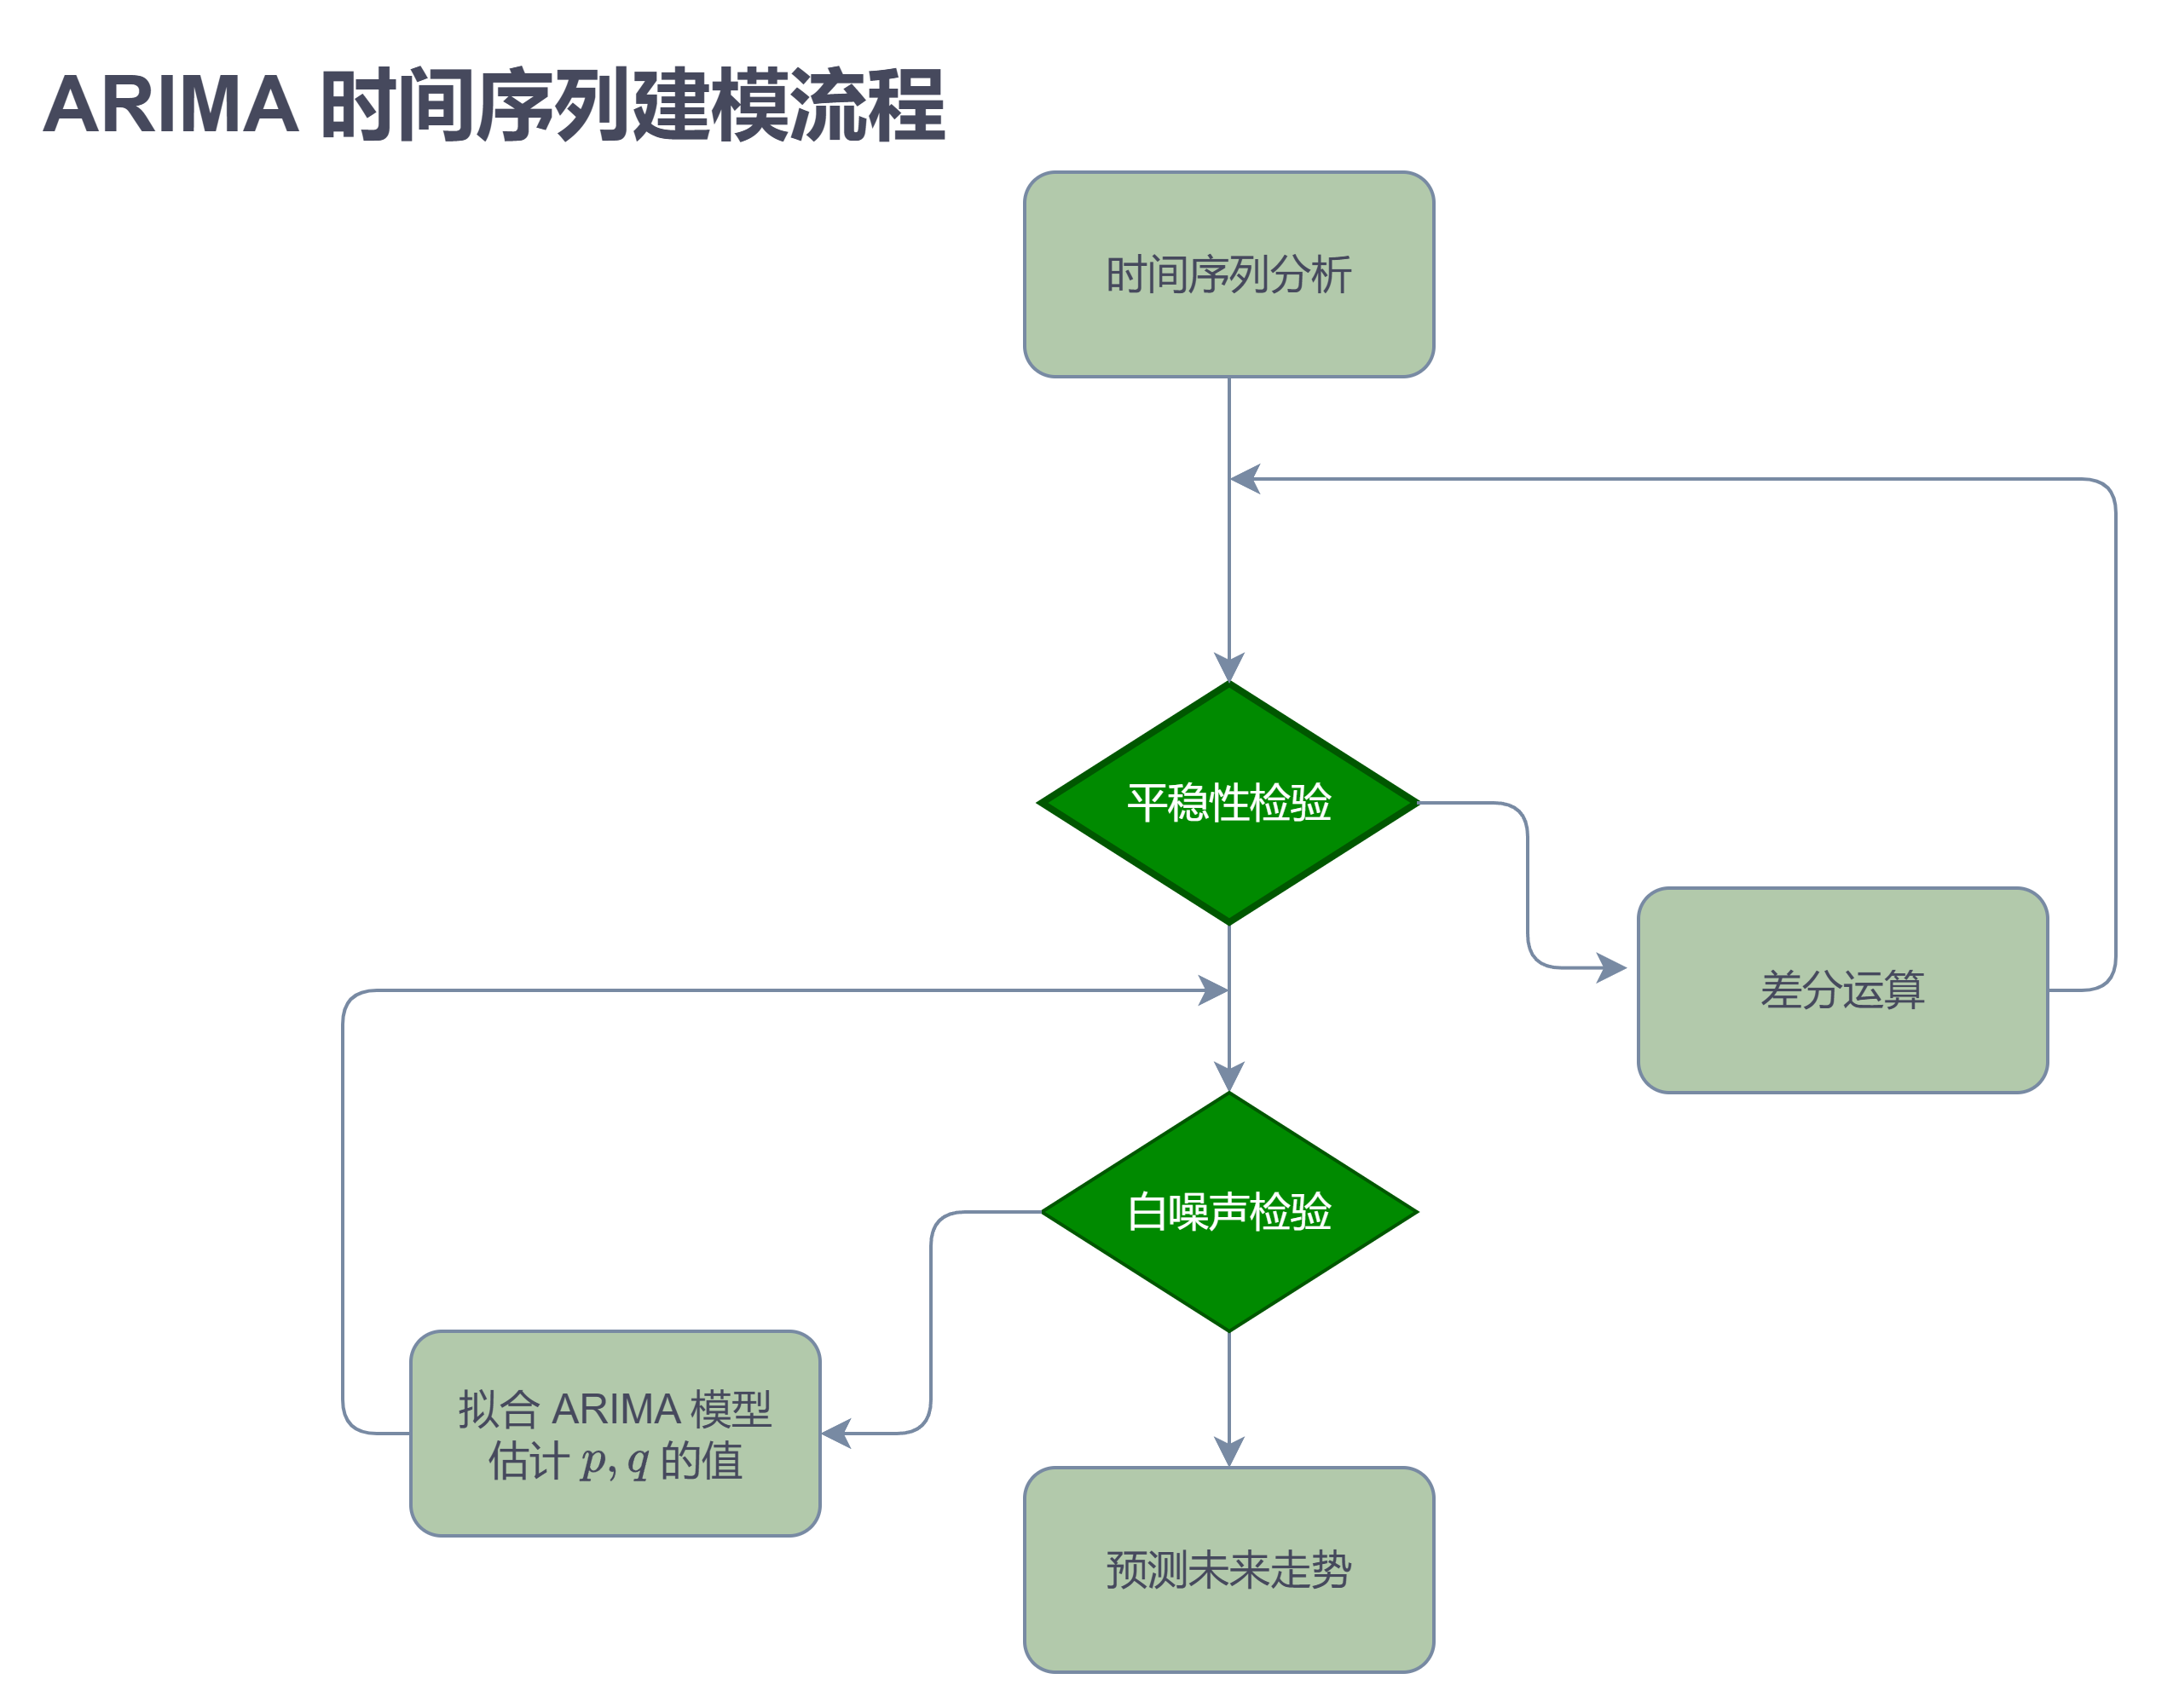
\includegraphics[width=0.6\textwidth]{chapters/时间序列/images/ARIMA/img-20250803004058.png}
\end{figure}

\begin{definition}[ARIMA 模型]
    ARIMA 的全称是自回归整合移动平均模型（AutoRegressive Integrated Moving Average），它是一种用于时间序列预测的统计模型。它有三个部分：
    \begin{enumerate}
        \item AR (自回归)：模型中包含数据过去的值。参数 $p$ 是自回归的阶数（这个参数由 PACF 图确定）。实际上，就是由一个基准值，确定了某些线性系数后，参考过去的值得到现在的值，即下述公式（线性模型一定存在误差 $\varepsilon_t$）：
              $$y_t=\mu+\sum_{i=1}^p r_i \cdot y_{t-1}+\varepsilon_t$$
        \item I (整合/差分)：为了让数据变得平稳而进行的差分次数。参数 $d$ 是差分的阶数。
        \item MA (移动平均)：为了解决线性模型中的误差，MA 就产生了，模型中包含了过去的预测误差。参数 $q$ 是移动平均的阶数（由 ACF 图确定）。将前面的预测产生的误差进行叠加，即：
              $$y_{t-4} y_{t-3} y_{t-2} y_{t-1} + \sum \theta_i \varepsilon_i = {y_t}$$
        \item 合体之后，就是 ARMA 模型：
              $$y_t=\mu+\sum_{i=1}^p \gamma_i y_{t-1}+\sum_{i=1}^q \theta_i \varepsilon_{t-1}$$
        \item 所以，建立一个 ARIMA 模型，我们最终需要确定 ($p$, $d$, $q$) 这三个参数。
    \end{enumerate}
\end{definition}

ARIMA 模型的执行流程可以分为以下几个步骤：

\begin{enumerate}
    \item 数据准备：创建一组有趋势和季节性的模拟时间序列数据。
    \item 平稳性检验：通过可视化和统计检验（ADF检验）判断序列是否平稳。
    \item 差分处理：对非平稳序列进行差分，使其平稳，并确定差分阶数 $d$。
    \item 模型定阶：使用 ACF 和 PACF 图来帮助确定 $p$ (自回归阶数) 和 $q$ (移动平均阶数)。
    \item 模型训练与预测：建立并训练 ARIMA 模型，然后进行预测。
    \item 结果可视化：将预测结果与真实值进行对比。
    \item 计算 RMSE：这个值越大，模型的性能就越好。
\end{enumerate}

\subsection{ARIMA 模型的执行步骤}

\subsubsection{平稳性检验}

拿到一个时间序列首先需要平稳性检验和白噪声检验（随机性检验），只有处理为平稳的非白噪声数据才能继续使用 ARIMA 模型进行预测。

\begin{lstlisting}[style=python]
ds = [10930, 10318, 10595, 10972, 7706, 6756, 9092, 10551, 9722, 10913, 11151, 8186, 6422,
      6337, 11649, 11652, 10310, 12043, 7937, 6476, 9662, 9570, 9981, 9331, 9449, 6773, 6304, 9355,
      10477, 10148, 10395, 11261, 8713, 7299, 10424, 10795, 11069, 11602, 11427, 9095, 7707, 10767,
      12136, 12812, 12006, 12528, 10329, 7818, 11719, 11683, 12603, 11495, 13670, 11337, 10232,
      13261, 13230, 15535, 16837, 19598, 14823, 11622, 19391, 18177, 19994, 14723, 15694, 13248,
      9543, 12872, 13101, 15053, 12619, 13749, 10228, 9725, 14729, 12518, 14564, 15085, 14722,
      11999, 9390, 13481, 14795, 15845, 15271, 14686, 11054, 10395]

# 原 Data Series
ds = pd.Series(ds)
ds.index = pd.Index(sm.tsa.datetools.dates_from_range('2001', '2090'))
ds.plot(figsize=(12, 8))
plt.title('dta')
\end{lstlisting}

\subsubsection{差分处理}

均值和方差差不多不变的，就算是平稳的。ARIMA 模型只能预测平稳的。
若不平稳，就进行 $n$ 阶差分。

\begin{lstlisting}[style=python]
dta_diff1 = ds.diff(1)
dta_diff1.dropna(inplace=True)
\end{lstlisting}

\subsubsection{ADF 平稳性检验}

\begin{enumerate}
    \item 要检验当前的数据序列是否平稳，除了观察\textbf{趋势}、\textbf{季节性}、\textbf{方差变化}之外，还可以通过单位根检验，在 ARIMA 模型中，通常使用\textbf{ADF 检验}。
\end{enumerate}

\begin{theorem}[ADF 检验]
    \begin{enumerate}
        \item 原假设 $H_0$：时间序列存在单位根（非平稳）。
        \item 备择假设 $H_1$：时间序列不存在单位根（平稳）。
        \item 通过计算ADF统计量并与临界值比较来进行检验。
    \end{enumerate}

    \begin{tips}
        \begin{enumerate}
            \item $P$ 值若 $ \leq 0.05$ （或自己选择更小的），则有充分的理由拒绝原假设，认为序列是平稳的。
            \item 如果 $P > 0.05$ ，则我们不能拒绝原假设，认为序列是非平稳的。
            \item ADF Test Statistic（ADF检验统计量）：
                  \begin{itemize}
                      \item 这是一个负数。如果这个值越小（越负），就越有理由拒绝原假设，认为数据是平稳的。
                      \item 需要将它与不同显著性水平下的 Critical Values（临界值）进行比较。如果 $\text{Test Statistic} < \text{Critical Value}$，则拒绝原假设，认为序列是平稳的。
                  \end{itemize}
        \end{enumerate}
    \end{tips}
\end{theorem}

在 Python 中使用 ADF 检验，可以使用 \verb`adfuller` 函数。

\begin{lstlisting}[style=python]
def test_stationarity(timeseries):
    # 计算滚动均值
    roll_mean = timeseries.rolling(20).mean()
    roll_std = timeseries.rolling(20).std()

    plt.figure(figsize=(10, 5))
    plt.plot(timeseries, color='blue', label='原序列')
    plt.plot(roll_mean, color='red', label='滚动均值')
    plt.plot(roll_std, color='black', label='滚动标准差')
    plt.legend(loc='best')
    plt.title('Rolling Mean & Standard Deviation')
    plt.show()

    # Perform Augmented-Dickey-Fuller Test:
    res = adfuller(timeseries, autolag='AIC') # 使用 AIC 准则选择滞后阶数
    print(f"ADF Value: {res[0]:.4f}, P: {res[1]:.8f}")
    for k, v in res[4].items():
        print('Critial Values:')
        print(f'   {k}, {v:.3f}')
    return res
\end{lstlisting}

此处，我们从 \verb`adfuller` 中获取 ADF 的值以及 Critical Value，ADF 值应该比 Critical Values 都小。

\begin{lstlisting}[style=python]
ADF Value: -4.9939, P: 0.00002282
Critial Values:
   1%, -3.519
Critial Values:
   5%, -2.900
Critial Values:
   10%, -2.587
\end{lstlisting}

\subsubsection{选择最佳的 $p$ 和 $q$ 参数}

完成上述步骤，我们就可以选择最佳的 $p$ 和 $q$ 参数的值了。此时需要获取平稳时间序列的自相关图和偏自相关图。

\begin{definition}[截尾和拖尾]
    \begin{itemize}
        \item 截尾：在大于某个常数后，快速地趋近于 0，则为 $k$ 阶截尾
        \item 拖尾：始终有非零值，不会在 $k$ 大于某个常数后就恒等于 0
    \end{itemize}
\end{definition}

\begin{figure} [H]
    \centering
    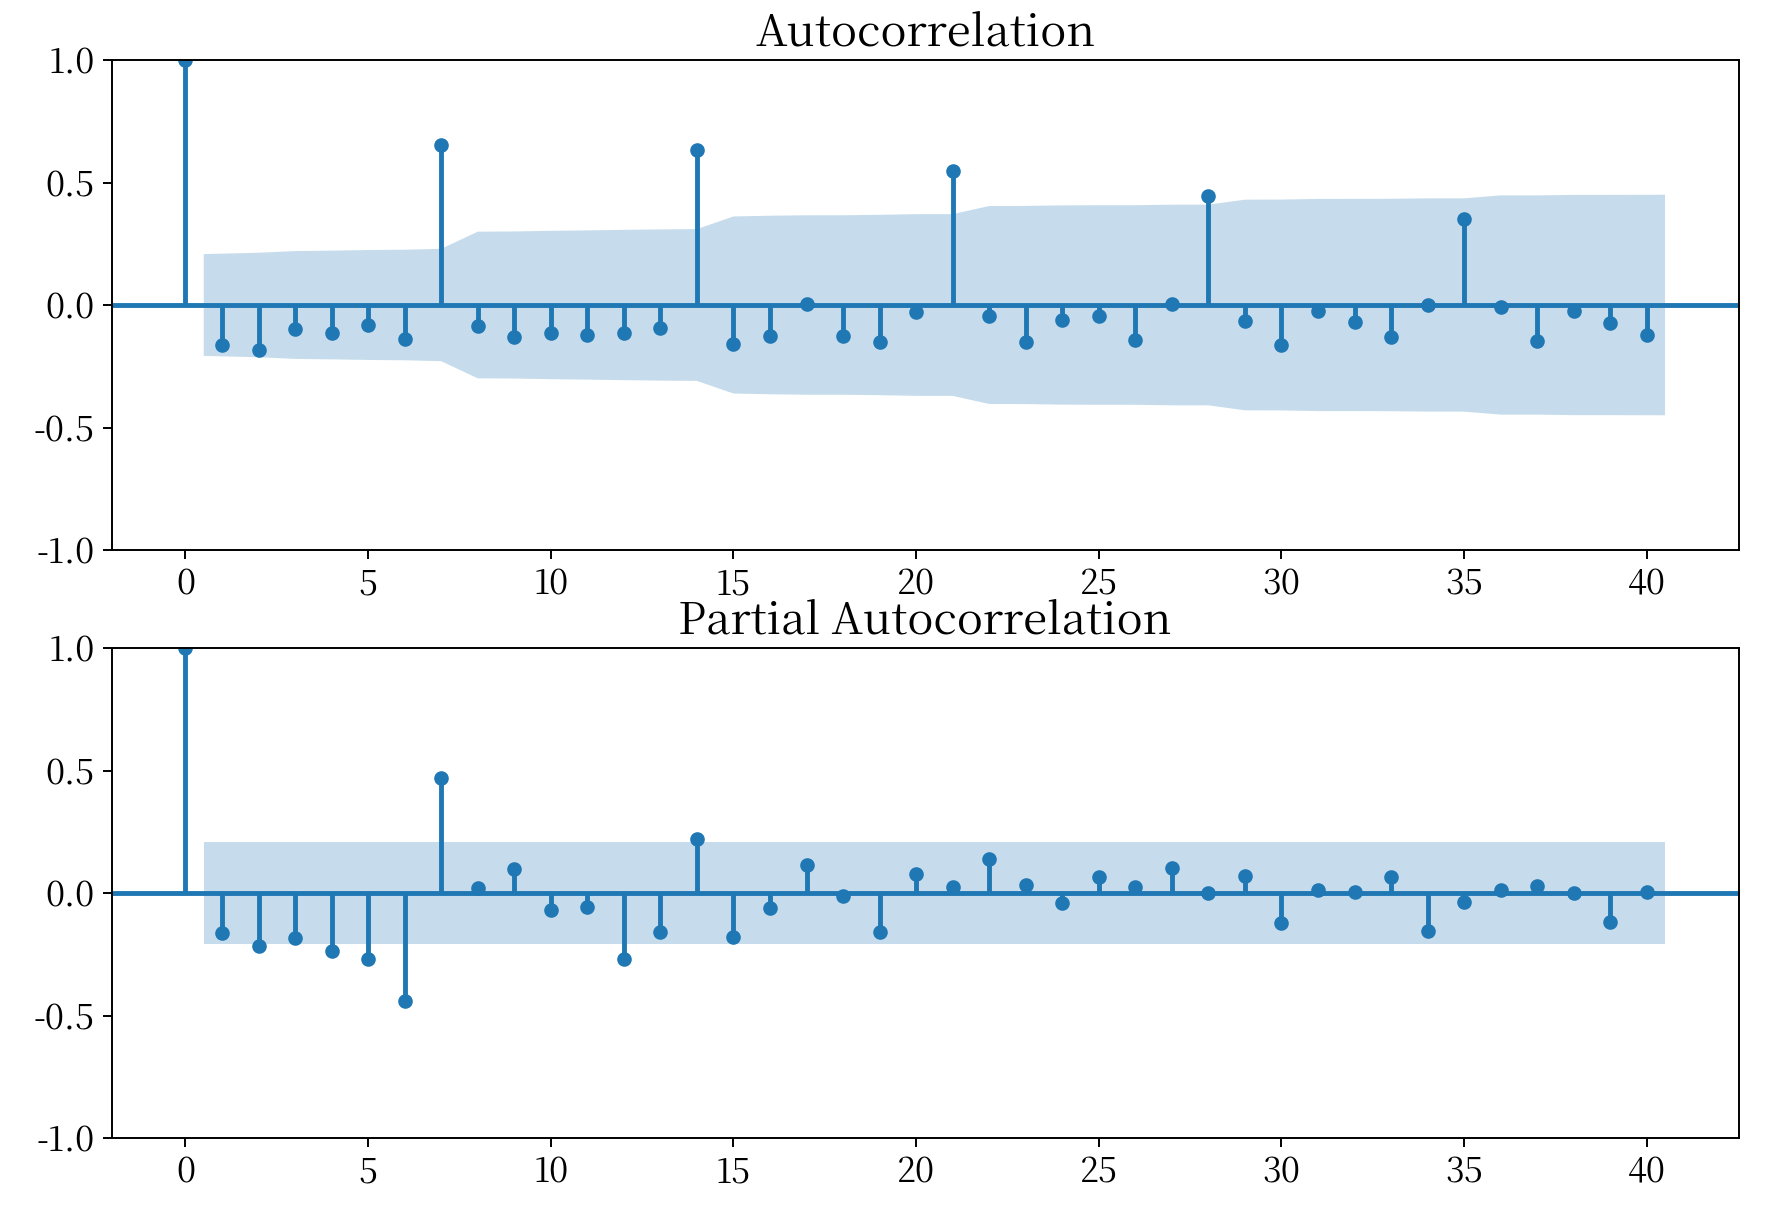
\includegraphics[width=0.5\textwidth]{chapters/时间序列/images/ARIMA/img-20250824215612.png}
\end{figure}

\begin{figure} [H]
    \centering
    \begin{tabular}{lll}
        \toprule
        模型            & 自相关系数（ACF） & 偏自相关系数（PACF） \\
        \midrule
        AR（$p$）       & 拖尾         & $P$ 阶截尾      \\
        MA（$q$）       & $q$ 阶截尾    & 拖尾           \\
        ARMA（$p$，$q$） & $p$ 阶拖尾    & $q$ 阶拖尾      \\
        \bottomrule
    \end{tabular}
    \caption{ARMA 模式识别原则}
\end{figure}

\begin{warning}
    若是双截尾，则序列本身不存在明显的自相关性，ARMA 类模型可能不适用。
\end{warning}

\begin{tips}
    这个图的读数法，置信区间是蓝色的部分，观察 PACF 图和 ACF 图呈现的是关系，从而确定符合什么模型，例如上图，两个都是拖尾，数据就可能符合 $ARMA(p,q)$ 模型，但是这种情况下，从图形中很难判断 $p$ 和 $q$ 的精确值。

    当然，如果是比较简单的：
    \begin{itemize}
        \item 如果 PACF 图呈现“截尾”，ACF 图呈现“拖尾”：强烈暗示数据符合 $AR(p)$ 模型。数出 PACF 图在哪一阶“截断”。例如，如果 PACF 在第 $2$ 阶之后的所有值都落入置信区间，那么 p 值就取 $2$。模型可以定为 $ARIMA(2, d, 0)$。
        \item 如果 ACF 图呈现“截尾”，PACF 图呈现“拖尾”：数据符合 MA(q) 模型。数出 ACF 图在哪一阶“截断”。例如，如果 ACF 在第 $1$ 阶之后的所有值都落入置信区间，那么 $q$ 值就取 $1$。模型可以定为 $ARIMA(0, d, 1)$。
    \end{itemize}
\end{tips}

\begin{figure} [H]
    \centering
    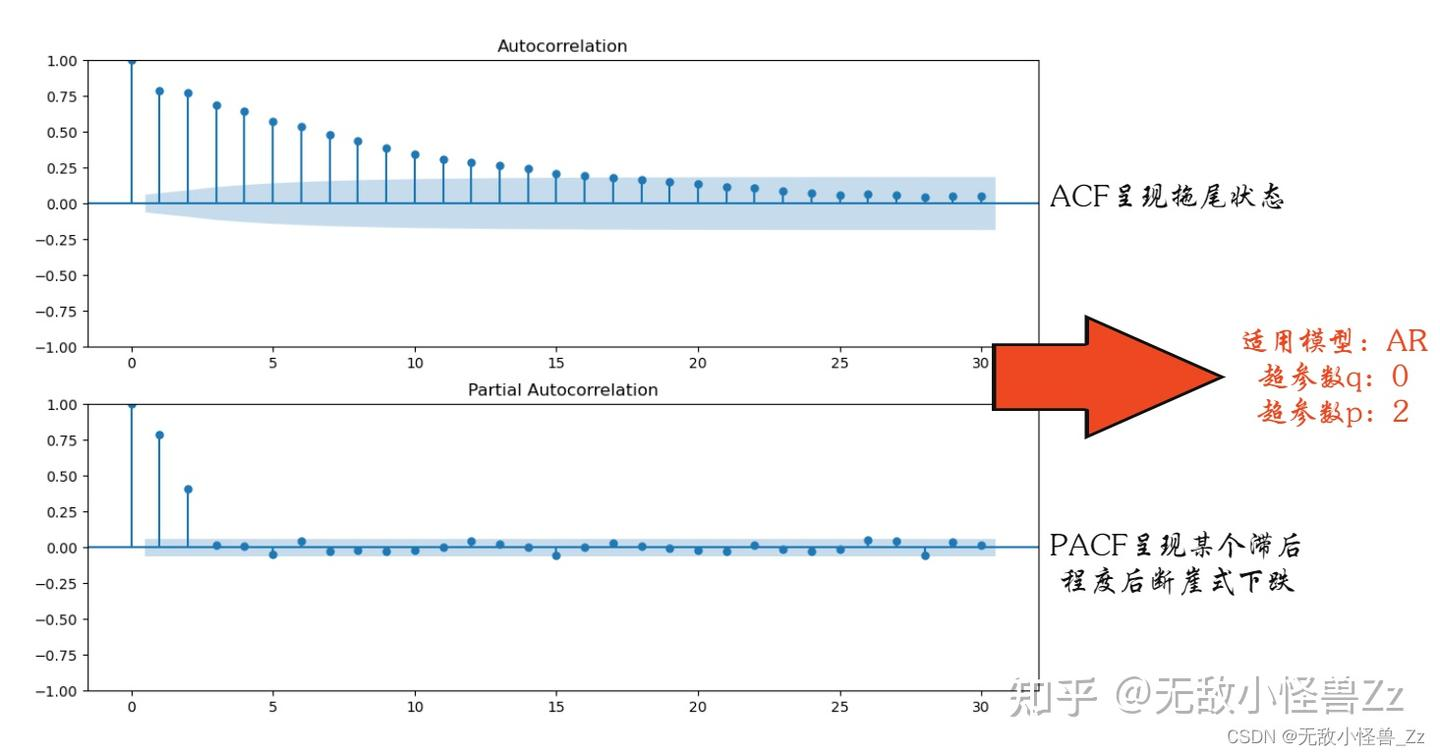
\includegraphics[width=0.65\textwidth]{chapters/时间序列/images/ARIMA/img-20250824230642.png}
\end{figure}

\begin{figure} [H]
    \centering
    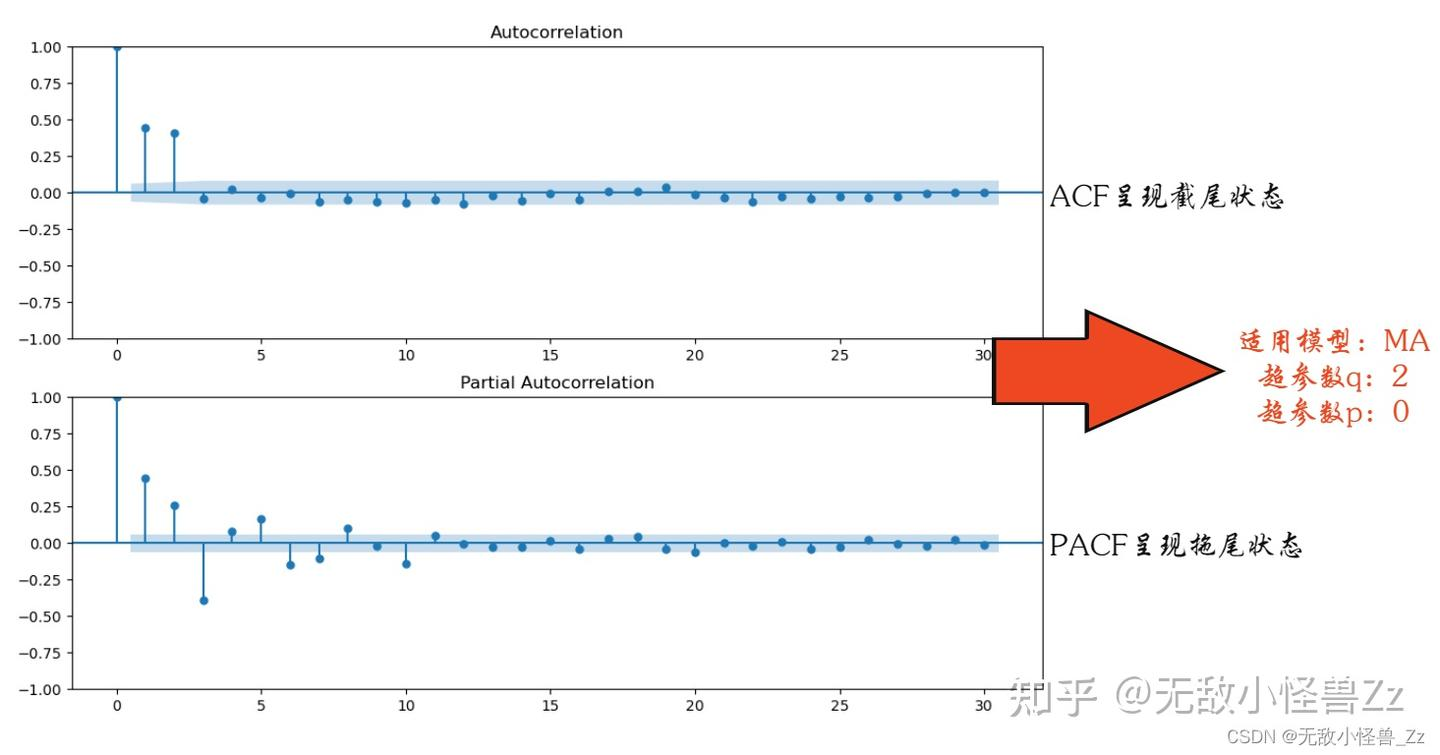
\includegraphics[width=0.65\textwidth]{chapters/时间序列/images/ARIMA/img-20250824230650.png}
\end{figure}


\subsubsection{信息准则定阶}

参考文献：\href{https://www.cnblogs.com/iupoint/p/14621830.html}{https://www.cnblogs.com/iupoint/p/14621830.html}

信息准则的好处是，在模型给出预测之前，就能对模型的超参做一个量化评估。

在批量预测的场景中尤其有用。因为批量预测往往需要程序在执行过程中自动确定阶数。

\begin{definition}[AIC 赤池信息准则]
    $$\mathrm{AIC}=-2 ln(L) +2(p+q+k+1)$$
    其中，$L$ 是模型的似然函数，$p$ 是自回归阶数，$q$ 是移动平均阶数，$k$ 是模型中参数的个数。$k = 1$ 表示模型考虑常数 $c$，$k=0$表示不考虑。最后一个 $1$ 表示算上误差项，所以第二项实际上就是 $2 \times \text{参数个数}$.

    而修正过的 $AICc$ 更好：

    $$
        \mathrm{AICc}=\mathrm{AIC}+\frac{2(p+q+k+1)(p+q+k+2)}{T-p-q-k-2}
    $$
\end{definition}

\begin{definition}[BIC 贝叶斯信息准则]
    $$
        \mathrm{BIC}=\mathrm{AIC}+[ln(T)-2](p+q+k+1)
    $$
\end{definition}

\begin{theorem}
    信息准则越小，说明参数的选择越好，一般就采用 $AICc$ 或者 $BIC$.
\end{theorem}

\begin{warning}
    差分量 $d$ 不要使用信息准则来判断，因为差分后会改变似然函数所使用的数据，信息的准则比较就失去了意义，所以先用其他的方法算出 $d$.
\end{warning}

\begin{warning}
    注意，AIC 和 BIC 信息量准则必须在原始数据上进行应用，所有参与比较的模型，必须是针对完全相同的观测数据计算出的似然函数 L。

    并且，这里会构造一个 $ARIMA(p,d,q)$ 模型，已经具备差分了。
\end{warning}

\begin{lstlisting}[style=python]
# 我们将行设置为 p (AR)，列设置为 q (MA)
aic_matrix = pd.DataFrame(index=[f'AR{i}' for i in range(p_max + 1)],
                          columns=[f'MA{i}' for i in range(q_max + 1)],
                          dtype=float)
bic_matrix = pd.DataFrame(index=[f'AR{i}' for i in range(p_max + 1)],
                          columns=[f'MA{i}' for i in range(q_max + 1)],
                          dtype=float)

for p in range(p_max + 1):
    for q in range(q_max + 1):
        # 避免拟合 ARIMA(0,1,0) 模型
        if p == 0 and q == 0:
            continue

        # 注意：我们是在原始序列 ds 上操作，并设置 d=1
        model = sm.tsa.ARIMA(ds, order=(p, 1, q))
        results = model.fit()

        # 将AIC和BIC存储到矩阵中
        aic_matrix.iloc[p, q] = results.aic
        bic_matrix.iloc[p, q] = results.bic
        print(f'完成: ARIMA({p}, 1, {q}) - AIC:{results.aic:.2f}, BIC:{results.bic:.2f}')
\end{lstlisting}

我们可以接着绘制 BIC 信息量的 HeatMap，这样能够可视化选取最优模型：

\begin{lstlisting}[style=python]
plt.figure(figsize=(10, 8))
sns.heatmap(bic_matrix.astype(float), annot=True, fmt=".2f", cmap="Purples")
plt.title('BIC (Bayesian Information Criterion) Heatmap')
plt.xlabel('MA order (q)')
plt.ylabel('AR order (p)')
plt.show()
\end{lstlisting}

\begin{figure} [H]
    \centering
    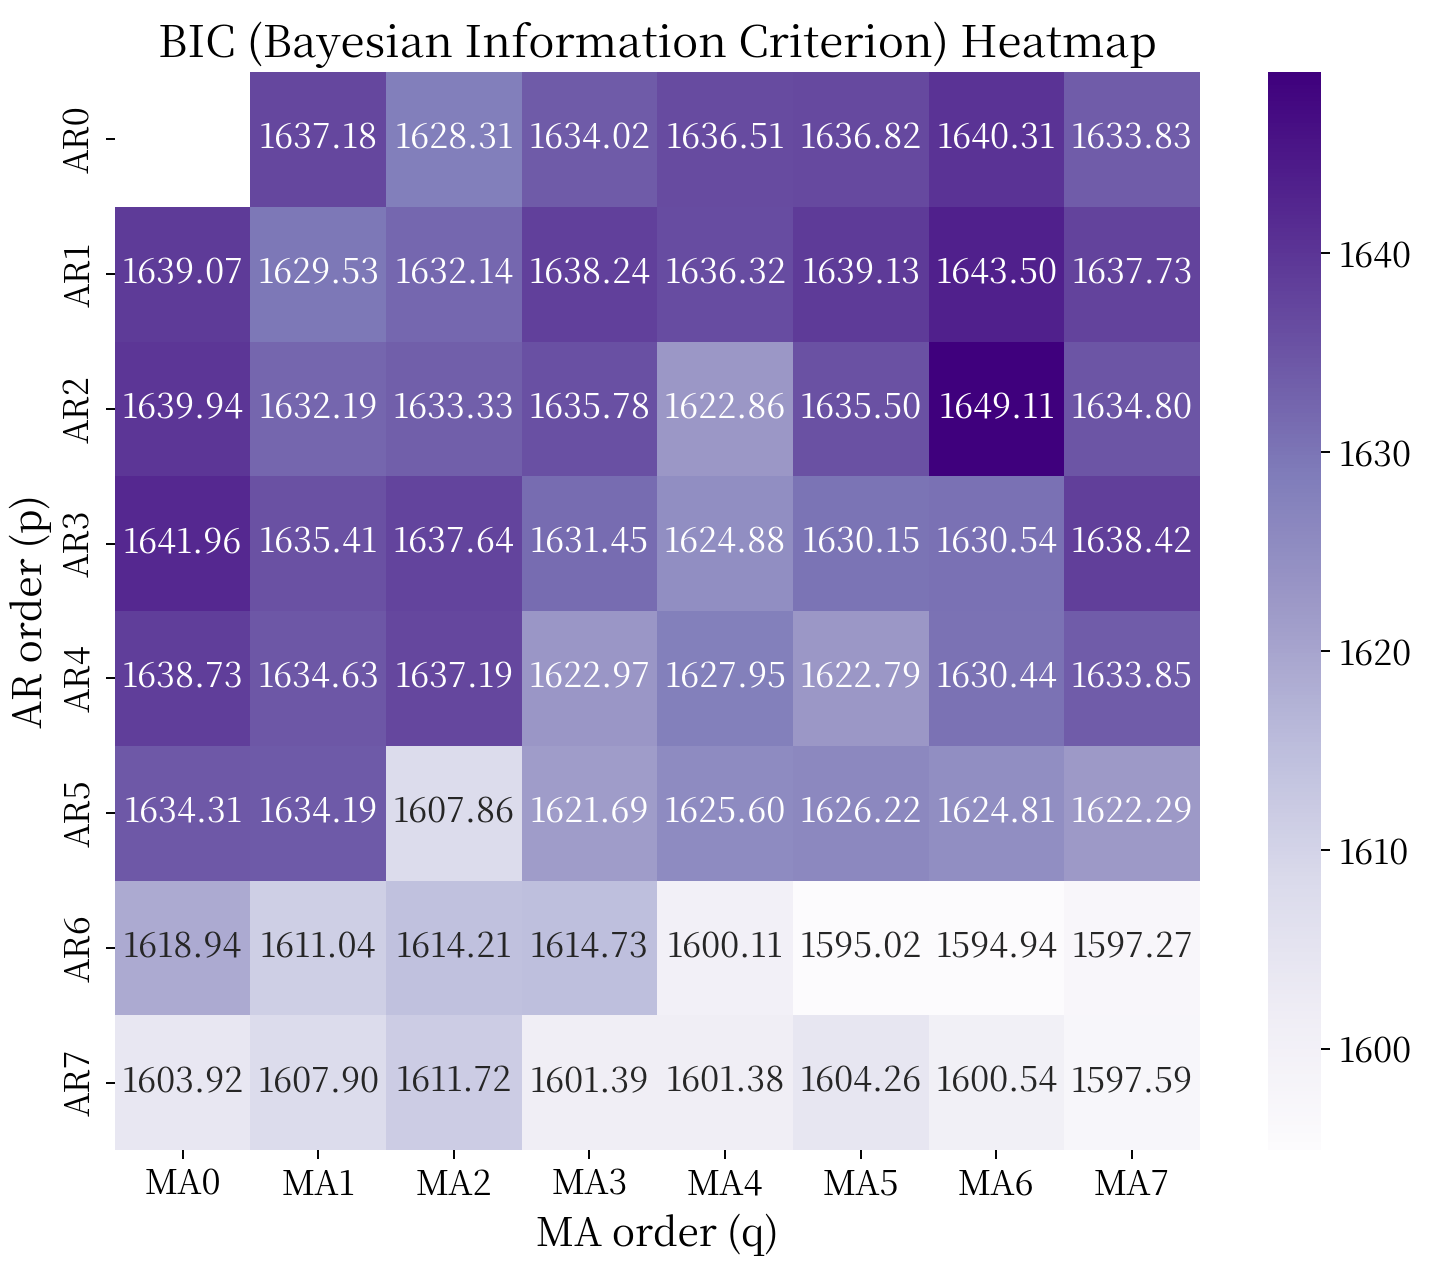
\includegraphics[width=0.45\textwidth]{chapters/时间序列/images/ARIMA/img-20250825002231.png}
\end{figure}

由图可知，我们可以选取 \verb`MA6,AR6` 模型进行 ARIMA 预测。这个 BIC 值是最小的。（BIC 值也可能是负值）

\subsubsection{模型初步构建}

\begin{lstlisting}[style=python]
# 构建 ARIMA 模型
model = sm.tsa.ARIMA(ds, order=(6,1,6))
results = model.fit()
pprint(results.summary())
\end{lstlisting}

这里的 Summary 结果可以为我们提供精简的信息。

\subsubsection{SARIMA 季节性周期模型}

如果后续发现有季节性周期变化，可以使用 SARIMA 模型。

\begin{lstlisting}[style=python]
# 使用 SARIMA 季节性模型
sarima_model = sm.tsa.SARIMAX(ds,order=(6, 1, 6),seasonal_order=(6, 1, 6, 7))
sarima_results = sarima_model.fit()
print(sarima_results.summary())
\end{lstlisting}

\subsubsection{模型检验}

\begin{definition}[QQ 图]
    QQ图用于直观验证一组数据是否来自某个分布，或者验证某两组数据是否来自同一（族）分布。

    QQ图是一种散点图，对应于正态分布的QQ图，就是由标准正态分布的分位数
    为横坐标，样本值为纵坐标的散点图。若 QQ 图上的点近似地在一条直线附近，说明是正态分布，而且该直线的斜率为标准差，截距为均值，用QQ图还
    可获得样本偏度和峰度的粗略信息。
\end{definition}

\begin{definition}[Ljung-Box 检验]
    判断模型的残差序列是否是白噪声（即完全随机，不存在任何自相关性）。一个好的模型，其残差必须是白噪声。

    LB检验则是基于一系列滞后阶数，判断序列总体的相关性或者说随机性是否存在。
    \begin{enumerate}
        \item 原假设 ($H_0$)：残差是白噪声。
        \item 我们希望得到的结果是无法拒绝原假设，即希望 $P > 0.05$。
    \end{enumerate}
\end{definition}

\begin{lstlisting}[style=python]
Ljung-Box Test on Residuals:
   lb_stat lb_pvalue
1  0.069148 0.792582
2  1.175858 0.555477
3  1.940543 0.584838
4  3.707892 0.446979
5  7.766225 0.169599
6  7.968889 0.240391
7 10.378889 0.168099
8 10.569353 0.227314
9 10.589831 0.304874
10 10.772259 0.375534
11 11.086204 0.436070
12 11.159994 0.515259
\end{lstlisting}

当所有的 $P$ 值都远远 $> 0.05$ 时，说明模型残差是纯粹的白噪声，模型已经成功提取了原始数据中所有的自相关（包括季节性）信息，没任何规律被遗漏。

\begin{definition}[D-W 检验]
    D-W 值显著接近于 $0$ 或 $4$ 时，则存在自相关性，而接近于 $2$ 时，则不存在（一阶）自相关性。
\end{definition}

\begin{figure} [H]
    \centering
    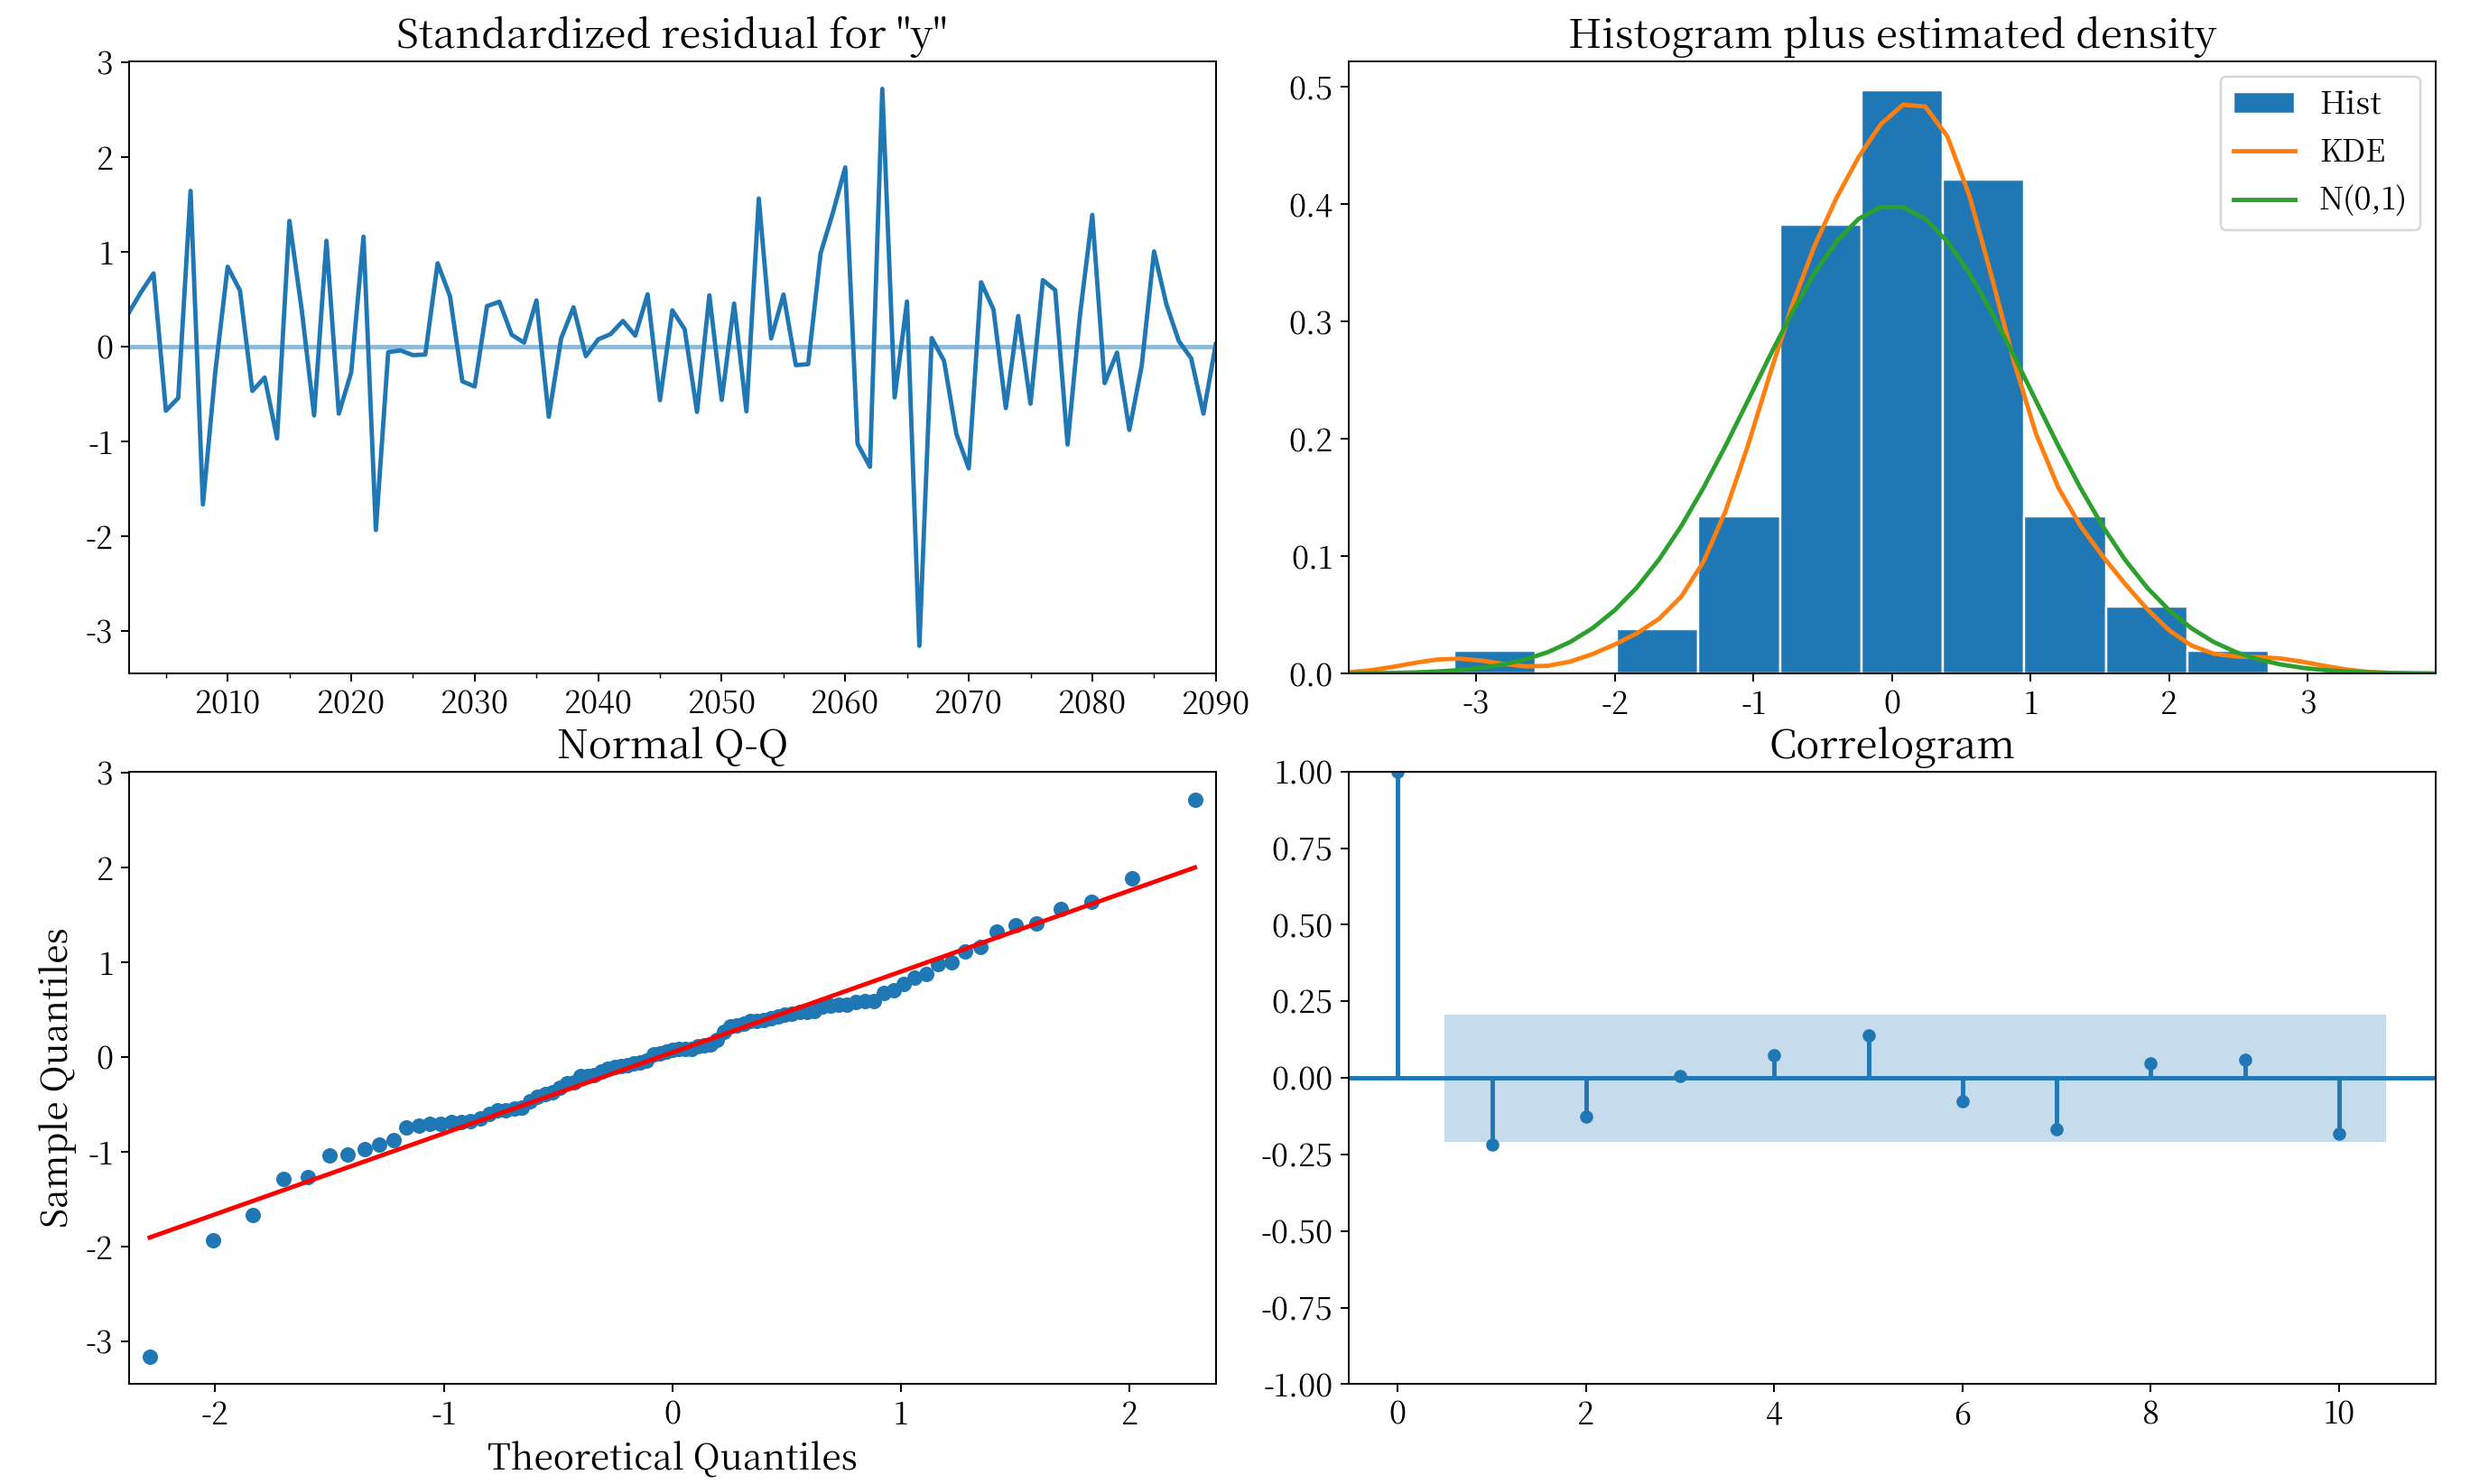
\includegraphics[width=0.8\textwidth]{chapters/时间序列/images/ARIMA/img-20250825015411.png}
\end{figure}

在构建完一个时间序列模型（如 ARIMA 或 SARIMA）后，我们必须对其进行模型诊断。

残差是模型的预测值与真实值之间的误差。一个好的模型，其残差序列应该表现为白噪声，即：
\begin{itemize}
    \item 均值为0，方差恒定（稳定性）。
    \item 不存在自相关性（独立性）。
    \item 服从正态分布（正态性）。
\end{itemize}

\verb`statsmodels` 库提供的标准四联诊断图正是围绕这几个核心假设进行检验的。

\subsubsection*{左上角：标准化残差图}

观察残差随时间的变化情况，用于直观判断残差序列是否稳定，是否存在异方差。

\begin{itemize}
    \item \textbf{理想情况：} 残差序列应在均值0的水平线上下随机、均匀地波动，没有显示出任何明显的趋势或周期性模式。同时，波动的幅度（方差）应该大致保持恒定。
    \item \textbf{问题情况：}
          \begin{itemize}
              \item 存在明显的上升或下降趋势、明显的周期性波动。
              \item 出现异方差性，例如波动的幅度随时间推移逐渐增大（呈喇叭口形状）或减小。
          \end{itemize}
\end{itemize}

\subsubsection*{右上角：直方图与核密度估计图}

检验残差的分布形态是否接近于正态分布。图中包含三条信息：
\begin{itemize}
    \item \textbf{蓝色直方图}: 残差数据的频数分布。
    \item \textbf{橙色KDE曲线}: 根据残差数据估计出的实际概率密度分布。
    \item \textbf{绿色N(0,1)曲线}: 标准正态分布的理论概率密度曲线。
\end{itemize}
\begin{itemize}
    \item \textbf{理想情况：} 橙色KDE曲线与绿色N(0,1)曲线应高度重合，且蓝色直方图的轮廓呈现对称的“钟形”。
    \item \textbf{问题情况：} 橙色曲线与绿色曲线形状差异巨大，或者直方图呈现明显的左偏或右偏形态。
\end{itemize}

\subsubsection*{左下角：正态 Q-Q 图}

通过比较残差的分位数与正态分布的分位数，更严谨地检验其正态性。

\begin{itemize}
    \item \textbf{理想情况：} 图中的蓝色数据点应基本紧密地排列在红色的对角线上。
    \item \textbf{问题情况：} 数据点系统性地偏离红线，形成“S”形、“弓”形或其他弯曲模式。
          \begin{itemize}
              \item \textbf{“肥尾” (Fat tails)}: 两端点向上和向下偏离红线，说明真实分布的尾部比正态分布更厚，存在更多极端值。
              \item \textbf{“瘦尾” (Thin tails)}: 两端点向红线内侧偏离。
          \end{itemize}
\end{itemize}

\subsubsection*{右下角：相关图 ACF}

检验残差中是否存在自相关性，这是判断残差是否为白噪声的最关键指标之一。

\begin{itemize}
    \item \textbf{理想情况：} 除了滞后阶数为0时（其值恒为1），其他所有滞后阶数的垂直线都应该落在蓝色的置信区间以内。
    \item \textbf{问题情况：} 有一根或多根垂直线显著地超出了蓝色置信区间的边界。这说明在对应的滞后阶数上存在显著的自相关，模型未能完全捕捉数据中的信息。
\end{itemize}

\subsection{ARIMA 模型的特例}

\begin{definition}[特例]
    \begin{enumerate}
        \item $\operatorname{ARIMA}(0,1,0)$ ：（此时当 $d=1, p$ 和 $q$ 为 0 时，称为 Random Walk 模型），该模型表示每一个时刻的位置，只与上一时刻的位置有关。
        \item $\operatorname{ARIMA}(1,0,0)$ ：（此时 $p=1, d=0, q=0$ ，称为 First-order Autoregressive Model），该模型说明时序数据是稳定的和自相关的。
        \item $\operatorname{ARIMA}(1,1,0)$ ：（此时 $p=1, d=1, q=0$ ，称为 Differenced First-order Autoregressive Model），该模型说明时序数据在一阶差分化之后是稳定的和自回归的，即一个时刻的差分（$y$）只与上一个时刻的差分有关。
        \item $\operatorname{ARIMA}(0,1,1)$ ：（此时 $p=0, d=1, q=1$ ，称为 Simple Exponential Smoothing With Growth 模型），该模型说明数据在一阶差分后是稳定的和移动平均的，即一个时刻的估计值的差分与上一个时刻的预测误差有关。
    \end{enumerate}
\end{definition}

